\subsection{Kiểm chứng thao tác quầy và realtime}
\begin{table}[htbp]\centering\small
\begin{tabularx}{\linewidth}{|p{.13\linewidth}|X|}\hline
\textbf{Ca} & \textbf{Điều kiện kiểm tra}\\\hline
QUAY-01 & Chỉ BARISTA vào staff API; không hiển thị đơn chưa trả/hủy trong hàng đợi pha.\\\hline
QUAY-02 & Đi đúng PAID--PREPARING--READY--COMPLETED; không tạo thêm Payment, trừ kho hoặc cộng điểm.\\\hline
QUAY-03 & Bỏ bước, lùi bước, bấm lặp và trạng thái/đầu vào sai bị từ chối.\\\hline
QUAY-04 & Hai nhân viên cùng duyệt một đơn: một response 200, một 409, trạng thái cuối nhất quán.\\\hline
QUAY-05 & Hai client WebSocket nhận sự kiện không payload sau commit, đọc API thấy trạng thái mới.\\\hline
QUAY-06 & Rollback và replay không phát thông báo thành công mới; hủy chỉ báo sau khi kho đã hoàn.\\\hline
QUAY-07 & Kết nối lại đọc được trạng thái mới; quyền đọc đơn cá nhân không bị mở rộng.\\\hline
QUAY-08 & Hàng đợi hơn 20 đơn vẫn giữ toàn bộ PAID/PREPARING/READY; nhóm hoàn tất giới hạn riêng.\\\hline
\end{tabularx}\caption{Các ca API và WebSocket cho quy trình quầy}
\end{table}

Các ca có tại \path{test/staff-orders.e2e-spec.ts}; bộ này có client Socket.IO kết nối thật tới ứng dụng test và đọc PostgreSQL để kiểm thứ tự commit/notify. Đây không chỉ là giả lập gọi một hàm emit. Các số liệu bộ hồi quy tham chiếu mục~\ref{sec:inventory-tests}; ảnh dưới sử dụng API fixture để minh họa bảng quầy, không tạo một kết quả chạy backend mới.

\begin{figure}[htbp]\centering
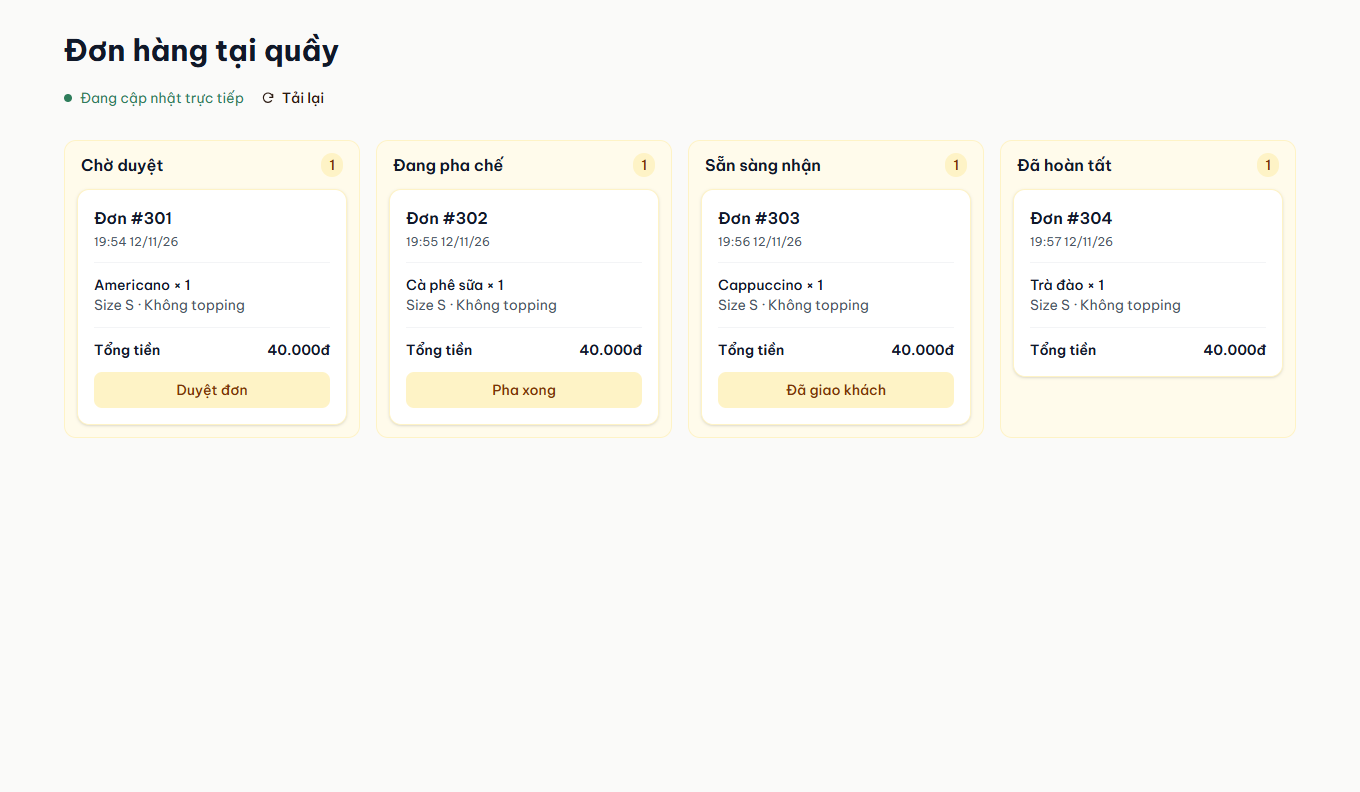
\includegraphics[width=.92\linewidth,height=.27\textheight,keepaspectratio]{assets/staff/board-ui-fixture.png}
\caption{Bốn cột xử lý đơn tại quầy với dữ liệu thử}
\end{figure}
